\section{طراحی مدل‌مبنا}
%مراحل طراحی و پیاده‌سازی براساس دیاگرام v (\ref{Vdiag}) طی می‌شود.
% با توجه به‌این دیاگرام، 
در طراحی مدل‌مبنا، ابتدا سامانه دینامیكی در محیط نرم‌افزاری مدل‌سازی و کنترل‌کننده طراحی می‌شود. سپس،  عملكرد کنترل‌کننده با استفاده از شبیه‌سازی نرم‌افزاری\LTRfootnote{MIL (Model In the Loop)} بررسی شده و اشكالات اولیه موجود برطرف می‌شود. در گام بعد، به‌منظور بررسی اثر نامعینی‌ها، ساده‌سازی‌ها و اشتباهات مدل‌سازی بر عملكرد کنترل‌کننده، شبیه‌سازی سخت‌افزار در حلقه پلنت\LTRfootnote{RCP (Rapid Control Prototyping)}
انجام می‌شود. پس از تایید عملكرد کنترل‌کننده به‌صورت نرم‌افزاری، کد آن به‌کمک ابزار تولید خودکار کد نرم‌افزار سیمولینک تولید و روی آردوینو\LTRfootnote{Arduino} پیاده‌سازی می‌شود.
% در این حالت، سخت‌افزار کنترل‌کننده (برد آردوینو) مدل در حلقه شبیه‌سازی قرار می‌گیرد.
 در مرحله نهایی، برد آردوینو به سامانه حقیقی (استند سه درجه آزادی) وصل شده، به‌صورت
زمان‌حقیقی\LTRfootnote{Real-Time} خروجی حسگر را دریافت و فرمان کنترلی را به سامانه اعمال می‌کند. در بخش‌های
\ref{quadall3}
و
\ref{parameeter_estimation_section}
به بررسی شبیه‌سازی و اصلاح پارامتر استند سه درجه آزادی چهارپره پرداخته می‌شود.
%\begin{figure}[H]
%	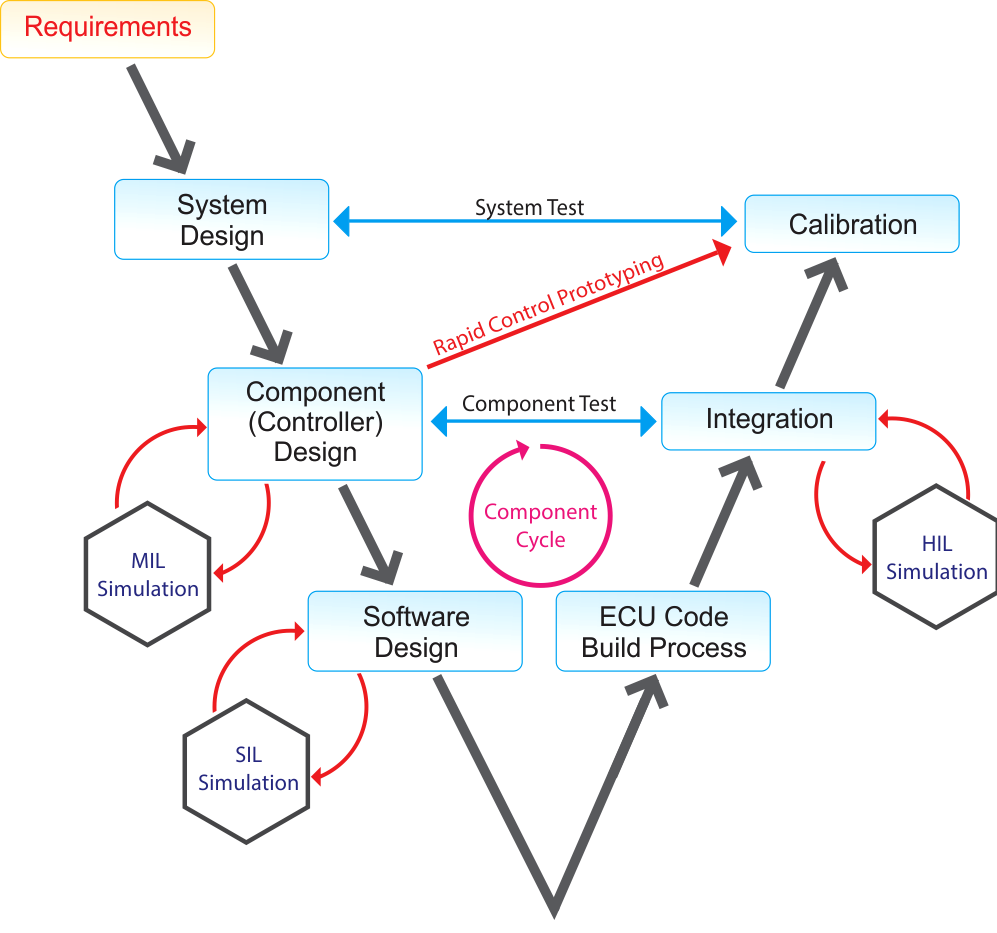
\includegraphics[width=10cm]{../Figures/QuadSimulation/ModelBasedDesign.png}
%	\centering
%	\caption{دیاگرام V 
%		\cite{Vdiagram}}
%	\label{Vdiag}
%\end{figure}